
\documentclass[ review  , 3p ]{elsarticle}
%default = preprint (single sapce), review = doublespace
%detail class option: https://www.elsevier.com/__data/assets/pdf_file/0008/56843/elsdoc-1.pdf

% eliminate "Preprinted to Elsevier"
\makeatletter
\def\ps@pprintTitle{%
 \let\@oddhead\@empty
 \let\@evenhead\@empty
 \def\@oddfoot{\centerline{\thepage}}%
 \let\@evenfoot\@oddfoot}
\makeatother

%%% Begin My package additions %%%%%%%%%%%%%%%%%%%
\usepackage[hyphens]{url}



\usepackage{lineno} % add
\providecommand{\tightlist}{%
  \setlength{\itemsep}{0pt}\setlength{\parskip}{0pt}}

\usepackage{graphicx}

\usepackage{zxjatype}
\usepackage{xeCJK}
\setCJKmainfont{ipaexm.ttf}
\setCJKsansfont{ipaexg.ttf}
\setCJKmonofont{ipaexg.ttf}

\usepackage{color}

\usepackage{booktabs}
\usepackage{longtable}
\usepackage{array}
\usepackage{multirow}
\usepackage{wrapfig}
\usepackage{float}
\usepackage{colortbl}
\usepackage{pdflscape}
\usepackage{tabu}
\usepackage{threeparttable}
\usepackage{threeparttablex}
\usepackage[normalem]{ulem}
\usepackage{makecell}
\usepackage{xcolor}


%\usepackage{xpatch}
%\xpatchcmd{\MaketitleBox}{\hrule}{}{}{}% remove first horizontal rule (above abstract)
%\xpatchcmd{\MaketitleBox}{\hrule}{}{}{}% remoce second horizonral rule (below keywords)
%%%%%%%%%%%%%%%% end my additions to header

\usepackage[T1]{fontenc}
\usepackage{lmodern}
\usepackage{amssymb,amsmath}
\usepackage{ifxetex,ifluatex}
\usepackage{fixltx2e} % provides \textsubscript
% use upquote if available, for straight quotes in verbatim environments
\IfFileExists{upquote.sty}{\usepackage{upquote}}{}
\ifnum 0\ifxetex 1\fi\ifluatex 1\fi=0 % if pdftex
  \usepackage[utf8]{inputenc}
\else % if luatex or xelatex
  \usepackage{fontspec}
  \ifxetex
    \usepackage{xltxtra,xunicode}
  \fi
  \defaultfontfeatures{Mapping=tex-text,Scale=MatchLowercase}
  \newcommand{\euro}{€}
\fi
% use microtype if available
\IfFileExists{microtype.sty}{\usepackage{microtype}}{}
\bibliographystyle{elsarticle-harvard}
\usepackage{tabularx}
\ifxetex
  \usepackage[setpagesize=false, % page size defined by xetex
              unicode=false, % unicode breaks when used with xetex
              xetex]{hyperref}
\else
  \usepackage[unicode=true]{hyperref}
\fi
\hypersetup{breaklinks=true,
            bookmarks=true,
            pdfauthor={},
            pdftitle={Short Paper},
            colorlinks=false,
            urlcolor=blue,
            linkcolor=magenta,
            pdfborder={0 0 0}}
\urlstyle{same}  % don't use monospace font for urls

\setcounter{secnumdepth}{5}

\newlength{\cslhangindent}
\setlength{\cslhangindent}{1.5em}
\newlength{\csllabelwidth}
\setlength{\csllabelwidth}{3em}
\newenvironment{CSLReferences}[3] % #1 hanging-ident, #2 entry spacing
 {% don't indent paragraphs
  \setlength{\parindent}{0pt}
  % turn on hanging indent if param 1 is 1
  \ifodd #1 \everypar{\setlength{\hangindent}{\cslhangindent}}\ignorespaces\fi
  % set entry spacing
  \ifnum #2 > 0
  \setlength{\parskip}{#2\baselineskip}
  \fi
 }%
 {}
\usepackage{calc} % for \widthof, \maxof
\newcommand{\CSLBlock}[1]{#1\hfill\break}
\newcommand{\CSLLeftMargin}[1]{\parbox[t]{\maxof{\widthof{#1}}{\csllabelwidth}}{#1}}
\newcommand{\CSLRightInline}[1]{\parbox[t]{\linewidth}{#1}}
\newcommand{\CSLIndent}[1]{\hspace{\cslhangindent}#1}

% Pandoc toggle for numbering sections (defaults to be off)


% Pandoc header


\begin{document}
  \begin{frontmatter}

    \title{Charitable Giving, Tax Reform, and Government Efficiency\tnoteref{1}}
            \tnotetext[1]{This research is base on}
                \author[Osaka University]{
      Hiroki Kato 
       \corref{*} }
     \ead{vge008kh@stundent.econ.osaka-u.ac.jp}   %to avoid auto-link, use \@ instead of @
        \author[Chiba University]{
      Tsuyoshi Goto 
      }
      %to avoid auto-link, use \@ instead of @
        \author[Kobe University]{
      Yong-Rok Kim 
      }
      %to avoid auto-link, use \@ instead of @
            \address[Osaka University]{Graduate School of Economics, Osaka University, Japan}
        \address[Chiba University]{Graduate School of Economics, Chiba University, Japan}
        \address[Kobe University]{Graduate School of Economics, Kobe University, Japan}
            \cortext[*]{Corresponding Author.}
      
        \begin{abstract}
      Brah
    \end{abstract}
      
        \begin{keyword}
      Charitable giving, Giving price, Tax reform, Governement efficiency, South Korea
       \JEL{D91, I10, I18} 
    \end{keyword}
    
  \end{frontmatter}

  \hypertarget{introduction}{%
  \section{Introduction}\label{introduction}}
  
  Placeholder
  
  \hypertarget{charitable-giving-and-taxiation}{%
  \subsection{Charitable Giving and Taxiation}\label{charitable-giving-and-taxiation}}
  
  \hypertarget{summary-in-short}{%
  \subsection{Summary in short}\label{summary-in-short}}
  
  \hypertarget{south-korean-tax-reform}{%
  \subsection{South Korean tax reform}\label{south-korean-tax-reform}}
  
  \hypertarget{related-literature}{%
  \subsection{Related Literature}\label{related-literature}}
  
  \hypertarget{research-about-tax-price-elasticity-of-charitable-donations}{%
  \subsection{Research about tax price elasticity of charitable donations}\label{research-about-tax-price-elasticity-of-charitable-donations}}
  
  \hypertarget{research-about-perception-towards-the-government-and-donationtax-payment.}{%
  \subsection{Research about perception towards the government and donation/tax payment.}\label{research-about-perception-towards-the-government-and-donationtax-payment.}}
  
  \hypertarget{why-political-trust}{%
  \subsection{Why Political Trust?}\label{why-political-trust}}
  
  \hypertarget{institutional-background}{%
  \section{Institutional background}\label{institutional-background}}
  
  Placeholder
  
  \hypertarget{tax-relief-for-charitable-giving-by-tax-deduction-and-tax-credit}{%
  \subsection{Tax relief for charitable giving by tax deduction and tax credit}\label{tax-relief-for-charitable-giving-by-tax-deduction-and-tax-credit}}
  
  \hypertarget{korean-tax-reform-in-2014-need-modification-by-kim-san}{%
  \subsection{Korean tax reform in 2014 (Need modification by Kim san)}\label{korean-tax-reform-in-2014-need-modification-by-kim-san}}
  
  \hypertarget{data}{%
  \section{Data}\label{data}}
  
  Placeholder
  
  \hypertarget{national-survey-of-tax-and-benefit-nastab}{%
  \subsection{National Survey of Tax and Benefit (NaSTaB)}\label{national-survey-of-tax-and-benefit-nastab}}
  
  \hypertarget{time-series-of-chariable-giving}{%
  \subsection{Time Series of Chariable Giving}\label{time-series-of-chariable-giving}}
  
  \hypertarget{summary-statistics}{%
  \subsection{Summary Statistics}\label{summary-statistics}}
  
  \hypertarget{what-is-giving-price}{%
  \subsection{What is Giving Price?}\label{what-is-giving-price}}
  
  \hypertarget{determination-of-tax-amount}{%
  \subsection{Determination of Tax Amount}\label{determination-of-tax-amount}}
  
  \hypertarget{derive-giving-price}{%
  \subsection{Derive Giving Price}\label{derive-giving-price}}
  
  \hypertarget{construct-giving-price}{%
  \subsection{Construct Giving Price}\label{construct-giving-price}}
  
  \hypertarget{income-distribution-and-giving-price}{%
  \subsection{Income Distribution and Giving Price}\label{income-distribution-and-giving-price}}
  
  \hypertarget{empirical-strategy}{%
  \subsection{Empirical Strategy}\label{empirical-strategy}}
  
  \hypertarget{intensive-margin-and-extensive-margin}{%
  \subsection{Intensive Margin and Extensive Margin}\label{intensive-margin-and-extensive-margin}}
  
  \hypertarget{main-results}{%
  \section{Main Results}\label{main-results}}
  
  Placeholder
  
  \hypertarget{price-and-income-elasticity}{%
  \subsection{Price and Income Elasticity}\label{price-and-income-elasticity}}
  
  \hypertarget{baseline-regressions-result}{%
  \subsection{Baseline Regressions: Result}\label{baseline-regressions-result}}
  
  \hypertarget{intensive-margin-and-extensive-margin-result}{%
  \subsection{Intensive Margin and Extensive Margin: Result}\label{intensive-margin-and-extensive-margin-result}}
  
  \hypertarget{robustness-check}{%
  \subsection{Robustness Check}\label{robustness-check}}
  
  \hypertarget{robustness-check-1}{%
  \subsection{Robustness Check 1}\label{robustness-check-1}}
  
  \hypertarget{robustness-check-1-result}{%
  \subsection{Robustness Check 1: Result}\label{robustness-check-1-result}}
  
  \hypertarget{robustness-check-1-intensive-and-extensive-margin}{%
  \subsection{Robustness Check 1: Intensive and Extensive Margin}\label{robustness-check-1-intensive-and-extensive-margin}}
  
  \hypertarget{robust-check-2}{%
  \subsection{Robust Check 2}\label{robust-check-2}}
  
  \hypertarget{robustness-check-2-result}{%
  \subsection{Robustness Check 2: Result}\label{robustness-check-2-result}}
  
  \hypertarget{robustness-check-2-intensive-and-extensive-margin}{%
  \subsection{Robustness Check 2: Intensive and Extensive Margin}\label{robustness-check-2-intensive-and-extensive-margin}}
  
  \hypertarget{governement-efficient-and-price-elasticity}{%
  \section{Governement Efficient and Price Elasticity}\label{governement-efficient-and-price-elasticity}}
  
  \begin{figure}
  
  {\centering 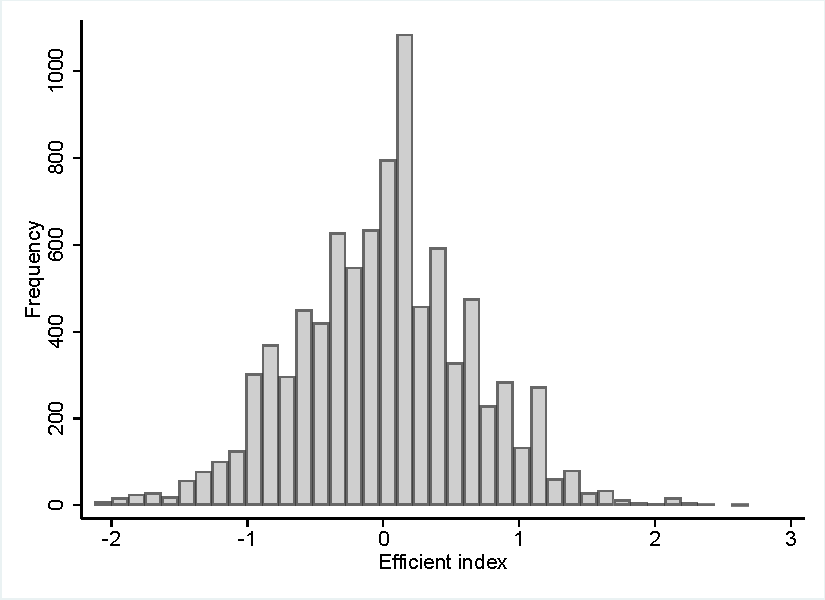
\includegraphics[width=0.9\linewidth]{C:/Users/vge00/Desktop/NaSTaB/_assets/HistogramEfficientid} 
  
  }
  
  \caption{Histogram of Efficient Index}\label{fig:unnamed-chunk-1}
  \end{figure}
  
  \begin{table}
  
  \caption{\label{tab:kableHeteroElasticity}Heterogenous Elasticity by Perceived Government Efficiency}
  \centering
  \fontsize{8}{10}\selectfont
  \begin{threeparttable}
  \begin{tabular}[t]{lccc}
  \toprule
  \multicolumn{1}{c}{ } & \multicolumn{1}{c}{Overall} & \multicolumn{1}{c}{Extensive} & \multicolumn{1}{c}{Intensive} \\
  \cmidrule(l{3pt}r{3pt}){2-2} \cmidrule(l{3pt}r{3pt}){3-3} \cmidrule(l{3pt}r{3pt}){4-4}
   & (1) & (2) & (3)\\
  \midrule
  ln(giving price) & -1.356*** & -0.284*** & -0.952***\\
   & (0.336) & (0.076) & (0.334)\\
  ln(giving price) X 2Q Efficient Group & -0.032 & -0.059 & 0.292\\
   & (0.423) & (0.098) & (0.489)\\
  ln(giving price) X 3Q Efficient Group & 0.353 & 0.095 & -0.285\\
   & (0.417) & (0.097) & (0.545)\\
  ln(auunaul taxable income) & 4.943*** & 1.104*** & 1.589**\\
   & (0.959) & (0.222) & (0.657)\\
  Implied price elasiticity (1Q efficient group) & -1.356*** & -1.396*** & -0.952***\\
   & (0.336) & (0.374) & (0.334)\\
  Implied price elasiticity (2Q efficient group) & -1.388*** & -1.686*** & -0.661*\\
   & (0.330) & (0.378) & (0.394)\\
  Implied price elasiticity (3Q efficient group) & -1.002*** & -0.930** & -1.237***\\
   & (0.327) & (0.374) & (0.468)\\
  Implied income elasticity & 4.943*** & 5.429*** & 1.589**\\
   & (0.959) & (1.093) & (0.657)\\
  Individual FE & Y & Y & Y\\
  Time FE & Y & Y & Y\\
  Other Controls & Y & Y & Y\\
  N & 50455 & 50455 & 11327\\
  R-sq & 0.020 & 0.020 & 0.034\\
  \bottomrule
  \end{tabular}
  \begin{tablenotes}
  \item Notes: $^{*}$ $p < 0.1$, $^{**}$ $p < 0.05$, $^{***}$ $p < 0.01$. Standard errors are clustered at individual level. The 2Q (3Q) Efficient Group is a dummy varaible taking 1 if individual $i$ belongs to the second (third) quanitle of efficient index. Other controls are age (its squared value), the interaction between year dummies and education dummies, the interaction between year dummies and gender dummies, and the interaction between year dummies and resident area. The implied extensive-margin elasticity is evaluated at the sample mean of $D_{ijt}$.
  \end{tablenotes}
  \end{threeparttable}
  \end{table}
  
  \begin{figure}
  
  {\centering 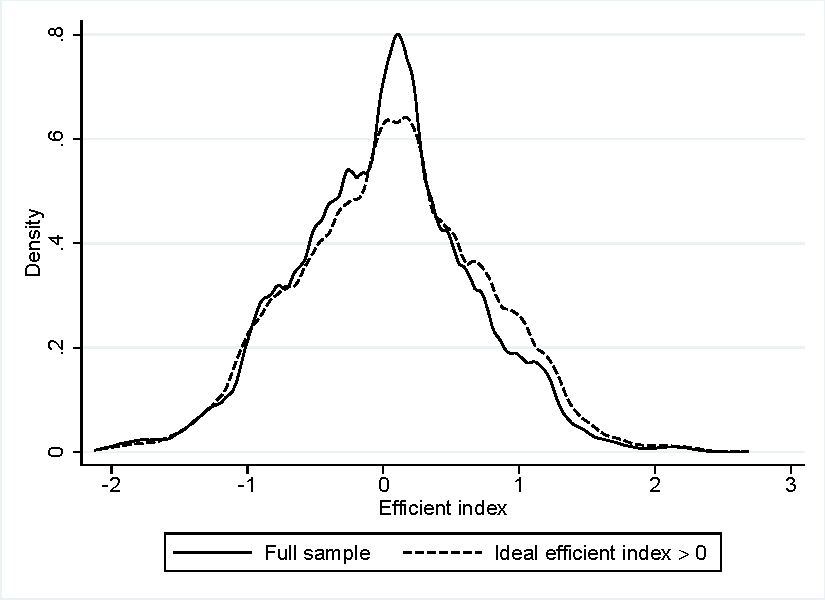
\includegraphics[width=0.9\linewidth]{C:/Users/vge00/Desktop/NaSTaB/_assets/DensityEfficientid} 
  
  }
  
  \caption{Density of Efficient Index Using those whose ideal efficient index > 0}\label{fig:unnamed-chunk-2}
  \end{figure}
  
  \begin{table}
  
  \caption{\label{tab:kableSubsetHeteroElasticity}Heterogenous Elasticity Using Those whose Ideal Efficient Index > 0}
  \centering
  \fontsize{8}{10}\selectfont
  \begin{threeparttable}
  \begin{tabular}[t]{lccc}
  \toprule
  \multicolumn{1}{c}{ } & \multicolumn{1}{c}{Overall} & \multicolumn{1}{c}{Extensive} & \multicolumn{1}{c}{Intensive} \\
  \cmidrule(l{3pt}r{3pt}){2-2} \cmidrule(l{3pt}r{3pt}){3-3} \cmidrule(l{3pt}r{3pt}){4-4}
   & (1) & (2) & (3)\\
  \midrule
  ln(giving price) & -1.831*** & -0.316*** & -1.303**\\
   & (0.538) & (0.115) & (0.571)\\
  ln(giving price) X 2Q Efficient Group & 0.339 & 0.045 & 0.308\\
   & (0.657) & (0.146) & (0.807)\\
  ln(giving price) X 3Q Efficient Group & 1.295** & 0.237* & 0.236\\
   & (0.586) & (0.135) & (0.834)\\
  ln(auunaul taxable income) & 5.686*** & 1.202*** & 3.225*\\
   & (1.272) & (0.273) & (1.880)\\
  Implied price elasiticity (1Q efficient group) & -1.831*** & -1.555*** & -1.303**\\
   & (0.538) & (0.565) & (0.571)\\
  Implied price elasiticity (2Q efficient group) & -1.492*** & -1.335** & -0.995\\
   & (0.505) & (0.561) & (0.622)\\
  Implied price elasiticity (3Q efficient group) & -0.536 & -0.392 & -1.067\\
   & (0.416) & (0.500) & (0.680)\\
  Implied income elasticity & 5.686*** & 5.913*** & 3.225*\\
   & (1.272) & (1.344) & (1.880)\\
  Individual FE & Y & Y & Y\\
  Time FE & Y & Y & Y\\
  Other Controls & Y & Y & Y\\
  N & 23366 & 23366 & 5004\\
  R-sq & 0.020 & 0.019 & 0.057\\
  \bottomrule
  \end{tabular}
  \begin{tablenotes}
  \item Notes: $^{*}$ $p < 0.1$, $^{**}$ $p < 0.05$, $^{***}$ $p < 0.01$. Standard errors are clustered at individual level. The 2Q (3Q) Efficient Group is a dummy varaible taking 1 if individual $i$ belongs to the second (third) quanitle of efficient index. Other controls are age (its squared value), the interaction between year dummies and education dummies, the interaction between year dummies and gender dummies, and the interaction between year dummies and resident area. We drop units whose the ideal efficient index is less than or equal to zero. The implied extensive-margin elasticity is evaluated at the sample mean of $D_{ijt}$.
  \end{tablenotes}
  \end{threeparttable}
  \end{table}
  
  \begin{table}
  
  \caption{\label{tab:kableHeteroLastElasticity}Heterogenous Last Price Elasticity: Panel IV}
  \centering
  \fontsize{8}{10}\selectfont
  \begin{threeparttable}
  \begin{tabular}[t]{lcccccc}
  \toprule
  \multicolumn{1}{c}{ } & \multicolumn{3}{c}{Full Sample} & \multicolumn{3}{c}{Ideal Efficient Index > 0} \\
  \cmidrule(l{3pt}r{3pt}){2-4} \cmidrule(l{3pt}r{3pt}){5-7}
  \multicolumn{1}{c}{ } & \multicolumn{1}{c}{Overall} & \multicolumn{1}{c}{Extensive} & \multicolumn{1}{c}{Intensive} & \multicolumn{1}{c}{Overall} & \multicolumn{1}{c}{Extensive} & \multicolumn{1}{c}{Intensive} \\
  \cmidrule(l{3pt}r{3pt}){2-2} \cmidrule(l{3pt}r{3pt}){3-3} \cmidrule(l{3pt}r{3pt}){4-4} \cmidrule(l{3pt}r{3pt}){5-5} \cmidrule(l{3pt}r{3pt}){6-6} \cmidrule(l{3pt}r{3pt}){7-7}
   & (1) & (2) & (3) & (4) & (5) & (6)\\
  \midrule
  ln(last giving price) & -2.604*** & -0.586*** & -1.166*** & -2.984*** & -0.579*** & -1.681**\\
   & (0.342) & (0.077) & (0.438) & (0.551) & (0.116) & (0.778)\\
  ln(last giving price) X 2Q Efficient Group & -0.272 & -0.104 & 0.043 & -0.108 & -0.063 & 0.239\\
   & (0.417) & (0.095) & (0.591) & (0.645) & (0.141) & (1.019)\\
  ln(last giving price) X 3Q Efficient Group & -0.010 & -0.038 & 0.111 & 0.894 & 0.056 & 1.285\\
   & (0.420) & (0.096) & (0.709) & (0.588) & (0.132) & (1.071)\\
  ln(auunaul taxable income) & 4.892*** & 1.087*** & 1.597** & 5.313*** & 1.141*** & 2.743\\
   & (0.958) & (0.222) & (0.670) & (1.282) & (0.277) & (1.947)\\
  Implied last price elasiticity (1Q efficient group) & -2.604*** & -2.883*** & -1.166*** & -2.984*** & -3.097*** & -1.681**\\
   & (0.342) & (0.377) & (0.438) & (0.551) & (0.621) & (0.778)\\
  Implied last price elasiticity (2Q efficient group) & -2.876*** & -3.395*** & -1.122** & -3.092*** & -3.432*** & -1.442*\\
   & (0.318) & (0.362) & (0.488) & (0.491) & (0.583) & (0.776)\\
  Implied last price elasiticity (3Q efficient group) & -2.614*** & -3.071*** & -1.055* & -2.091*** & -2.796*** & -0.396\\
   & (0.328) & (0.371) & (0.639) & (0.414) & (0.533) & (0.892)\\
  Implied income elasticity & 4.892*** & 5.345*** & 1.597** & 5.313*** & 6.097*** & 2.743\\
   & (0.958) & (1.094) & (0.670) & (1.282) & (1.481) & (1.947)\\
  Individual FE & Y & Y & Y & Y & Y & Y\\
  Time FE & Y & Y & Y & Y & Y & Y\\
  Other Controls & Y & Y & Y & Y & Y & Y\\
  N & 49575 & 49575 & 10447 & 22974 & 22974 & 4612\\
  \bottomrule
  \end{tabular}
  \begin{tablenotes}
  \item Notes: $^{*}$ $p < 0.1$, $^{**}$ $p < 0.05$, $^{***}$ $p < 0.01$. Standard errors are clustered at individual level. The 2Q (3Q) Efficient Group is a dummy varaible taking 1 if individual $i$ belongs to the second (third) quanitle of efficient index. Other controls are age (its squared value), the interaction between year dummies and education dummies, the interaction between year dummies and gender dummies, and the interaction between year dummies and resident area. The instumental variables are the first giving price in year $t$ and its interaction with the 2Q (3Q) Efficient Group. We drop units whose the ideal efficient index is less than or equal to zero in column (4)-(6). The implied extensive-margin elasticity is evaluated at the sample mean of $D_{ijt}$.
  \end{tablenotes}
  \end{threeparttable}
  \end{table}
  
  \begin{table}
  
  \caption{\label{tab:kableHeteroShortElasticity}Heterogenous Price Elasticity with Data after 2012}
  \centering
  \fontsize{8}{10}\selectfont
  \begin{threeparttable}
  \begin{tabular}[t]{lcccccc}
  \toprule
  \multicolumn{1}{c}{ } & \multicolumn{3}{c}{Full Sample} & \multicolumn{3}{c}{Ideal Efficient Index > 0} \\
  \cmidrule(l{3pt}r{3pt}){2-4} \cmidrule(l{3pt}r{3pt}){5-7}
  \multicolumn{1}{c}{ } & \multicolumn{1}{c}{Overall} & \multicolumn{1}{c}{Extensive} & \multicolumn{1}{c}{Intensive} & \multicolumn{1}{c}{Overall} & \multicolumn{1}{c}{Extensive} & \multicolumn{1}{c}{Intensive} \\
  \cmidrule(l{3pt}r{3pt}){2-2} \cmidrule(l{3pt}r{3pt}){3-3} \cmidrule(l{3pt}r{3pt}){4-4} \cmidrule(l{3pt}r{3pt}){5-5} \cmidrule(l{3pt}r{3pt}){6-6} \cmidrule(l{3pt}r{3pt}){7-7}
   & (1) & (2) & (3) & (4) & (5) & (6)\\
  \midrule
  ln(giving price) & -1.116*** & -0.197** & -1.175*** & -1.526** & -0.187 & -1.301*\\
   & (0.425) & (0.096) & (0.380) & (0.650) & (0.146) & (0.713)\\
  ln(giving price) X 2Q Efficient Group & -0.499 & -0.198 & 0.164 & 0.064 & -0.090 & -0.094\\
   & (0.544) & (0.124) & (0.558) & (0.863) & (0.192) & (0.974)\\
  ln(giving price) X 3Q Efficient Group & -0.125 & -0.060 & -0.167 & 0.448 & -0.036 & 0.197\\
   & (0.530) & (0.124) & (0.630) & (0.733) & (0.175) & (0.941)\\
  ln(auunaul taxable income) & 4.777*** & 1.034*** & 1.757*** & 6.126*** & 1.239*** & 2.903\\
   & (1.002) & (0.229) & (0.652) & (1.414) & (0.305) & (2.188)\\
  Implied price elasiticity (1Q efficient group) & -1.116*** & -0.951** & -1.175*** & -1.526** & -1.000 & -1.301*\\
   & (0.425) & (0.464) & (0.380) & (0.650) & (0.780) & (0.713)\\
  Implied price elasiticity (2Q efficient group) & -1.615*** & -1.910*** & -1.011** & -1.462** & -1.480* & -1.394*\\
   & (0.431) & (0.470) & (0.455) & (0.730) & (0.835) & (0.755)\\
  Implied price elasiticity (3Q efficient group) & -1.240*** & -1.242*** & -1.342** & -1.078* & -1.193* & -1.103\\
   & (0.413) & (0.470) & (0.549) & (0.550) & (0.722) & (0.739)\\
  Implied income elasticity & 4.777*** & 4.998*** & 1.757*** & 6.126*** & 6.622*** & 2.903\\
   & (1.002) & (1.107) & (0.652) & (1.414) & (1.632) & (2.188)\\
  Individual FE & Y & Y & Y & Y & Y & Y\\
  Time FE & Y & Y & Y & Y & Y & Y\\
  Other Controls & Y & Y & Y & Y & Y & Y\\
  N & 44115 & 44115 & 9967 & 20441 & 20441 & 4419\\
  R-sq & 0.018 & 0.019 & 0.034 & 0.018 & 0.018 & 0.061\\
  \bottomrule
  \end{tabular}
  \begin{tablenotes}
  \item Notes: $^{*}$ $p < 0.1$, $^{**}$ $p < 0.05$, $^{***}$ $p < 0.01$. Standard errors are clustered at individual level. The 2Q (3Q) Efficient Group is a dummy varaible taking 1 if individual $i$ belongs to the second (third) quanitle of efficient index. Other controls are age (its squared value), the interaction between year dummies and education dummies, the interaction between year dummies and gender dummies, and the interaction between year dummies and resident area. We drop units whose the ideal efficient index is less than or equal to zero in column (4)-(6). The implied extensive-margin elasticity is evaluated at the sample mean of $D_{ijt}$.
  \end{tablenotes}
  \end{threeparttable}
  \end{table}
  
  \begin{table}
  
  \caption{\label{tab:kableHeterokDiffElasticity}Heterogenous Price Elasticity: $k$-difference Model}
  \centering
  \fontsize{8}{10}\selectfont
  \begin{threeparttable}
  \begin{tabular}[t]{lcccccc}
  \toprule
  \multicolumn{1}{c}{ } & \multicolumn{3}{c}{Overall Elasticity} & \multicolumn{3}{c}{Intensive-Margin Elasticity} \\
  \cmidrule(l{3pt}r{3pt}){2-4} \cmidrule(l{3pt}r{3pt}){5-7}
  \multicolumn{1}{c}{Lag $k$} & \multicolumn{1}{c}{$k = 1$} & \multicolumn{1}{c}{$k = 2$} & \multicolumn{1}{c}{$k = 3$} & \multicolumn{1}{c}{$k = 1$} & \multicolumn{1}{c}{$k = 2$} & \multicolumn{1}{c}{$k = 3$} \\
  \cmidrule(l{3pt}r{3pt}){1-1} \cmidrule(l{3pt}r{3pt}){2-2} \cmidrule(l{3pt}r{3pt}){3-3} \cmidrule(l{3pt}r{3pt}){4-4} \cmidrule(l{3pt}r{3pt}){5-5} \cmidrule(l{3pt}r{3pt}){6-6} \cmidrule(l{3pt}r{3pt}){7-7}
   & (1) & (2) & (3) & (4) & (5) & (6)\\
  \midrule
  Lagged difference of first price (log) & -1.778*** & -2.884*** & -2.467*** & -1.401 & -2.320** & -2.549***\\
   & (0.553) & (0.520) & (0.509) & (1.074) & (0.970) & \vphantom{1} (0.788)\\
  \hspace{1em}X 2Q Efficient Group & -0.204 & 0.970 & 0.755 & -0.113 & -0.035 & 0.942\\
   & (0.747) & (0.687) & (0.648) & (1.548) & (1.331) & (1.128)\\
  \hspace{1em}X 3Q Efficient Group & -0.346 & 1.316** & 1.440** & -1.439 & 0.218 & 0.302\\
   & (0.704) & (0.644) & (0.624) & (1.610) & (1.319) & (1.196)\\
  Lagged difference of annual income (log) & 2.685** & 4.641*** & 5.274*** & 2.208 & 4.849*** & 5.471**\\
   & (1.045) & (1.149) & (1.185) & (1.712) & (1.816) & \vphantom{1} (2.189)\\
  Implied price elasiticity (1Q efficient group) & -1.778*** & -2.884*** & -2.467*** & -1.401 & -2.320** & -2.549***\\
   & (0.553) & (0.520) & (0.509) & (1.074) & (0.970) & (0.788)\\
  Implied price elasiticity (2Q efficient group) & -1.982*** & -1.914*** & -1.712*** & -1.515 & -2.355** & -1.607*\\
   & (0.611) & (0.546) & (0.508) & (1.230) & (0.986) & (0.885)\\
  Implied price elasiticity (3Q efficient group) & -2.123*** & -1.568*** & -1.027** & -2.840** & -2.102** & -2.248**\\
   & (0.550) & (0.494) & (0.485) & (1.317) & (0.995) & (0.973)\\
  Implied income elasticity & 2.685** & 4.641*** & 5.274*** & 2.208 & 4.849*** & 5.471**\\
   & (1.045) & (1.149) & (1.185) & (1.712) & (1.816) & (2.189)\\
  Individual FE & Y & Y & Y & Y & Y & Y\\
  Time FE & Y & Y & Y & Y & Y & Y\\
  Other Controls & Y & Y & Y & Y & Y & Y\\
  N & 46661 & 44448 & 42198 & 10675 & 10257 & 9811\\
  R-sq & 0.010 & 0.016 & 0.015 & 0.066 & 0.073 & 0.055\\
  \bottomrule
  \end{tabular}
  \begin{tablenotes}
  \item Notes: $^{*}$ $p < 0.1$, $^{**}$ $p < 0.05$, $^{***}$ $p < 0.01$. Standard errors are clustered at individual level. The 2Q (3Q) Efficient Group is a dummy varaible taking 1 if individual $i$ belongs to the second (third) quanitle of efficient index. The lagged difference of first price (log) is $\ln(\text{Price}^k_{ijt}) - \ln(\text{Price}_{ij(t-k)})$, where $\text{Price}^k_{ijt}$ calculates the giving price under the tax system in year $t$, using annual taxable income in year $t-k$, $\text{Income}_{ij(t-k)}$. The lagged of annual income (log) is $\ln(\text{Income}_{ijt}) - \ln(\text{Income}_{ij(t-k)})$. Other controls are lagged difference of age, lagged difference of squared age, the interaction between year dummies and education dummies, the interaction between year dummies and gender dummies, and the interaction between year dummies and resident area.
  \end{tablenotes}
  \end{threeparttable}
  \end{table}
  
  \begin{table}
  
  \caption{\label{tab:kableSubsetHeterokDiffElasticity}Heterogenous Price Elasticity: $k$-difference Model Using Those whose Ideal Efficient Index > 0}
  \centering
  \fontsize{8}{10}\selectfont
  \begin{threeparttable}
  \begin{tabular}[t]{lcccccc}
  \toprule
  \multicolumn{1}{c}{ } & \multicolumn{3}{c}{Overall Elasticity} & \multicolumn{3}{c}{Intensive-Margin Elasticity} \\
  \cmidrule(l{3pt}r{3pt}){2-4} \cmidrule(l{3pt}r{3pt}){5-7}
  \multicolumn{1}{c}{Lag $k$} & \multicolumn{1}{c}{$k = 1$} & \multicolumn{1}{c}{$k = 2$} & \multicolumn{1}{c}{$k = 3$} & \multicolumn{1}{c}{$k = 1$} & \multicolumn{1}{c}{$k = 2$} & \multicolumn{1}{c}{$k = 3$} \\
  \cmidrule(l{3pt}r{3pt}){1-1} \cmidrule(l{3pt}r{3pt}){2-2} \cmidrule(l{3pt}r{3pt}){3-3} \cmidrule(l{3pt}r{3pt}){4-4} \cmidrule(l{3pt}r{3pt}){5-5} \cmidrule(l{3pt}r{3pt}){6-6} \cmidrule(l{3pt}r{3pt}){7-7}
   & (1) & (2) & (3) & (4) & (5) & (6)\\
  \midrule
  Lagged difference of first price (log) & -2.215** & -3.269*** & -2.647*** & -0.841 & -4.928*** & -2.227\\
   & (0.872) & (0.794) & (0.821) & (1.936) & (1.780) & \vphantom{1} (1.588)\\
  \hspace{1em}X 2Q Efficient Group & 0.078 & 0.900 & 0.604 & -0.752 & 1.312 & -0.954\\
   & (1.233) & (1.070) & (0.972) & (2.841) & (2.329) & (1.992)\\
  \hspace{1em}X 3Q Efficient Group & -0.666 & 2.307*** & 2.242** & -3.101 & 3.154 & 2.071\\
   & (1.024) & (0.894) & (0.875) & (2.646) & (2.219) & (2.081)\\
  Lagged difference of annual income (log) & 3.048** & 5.197*** & 5.749*** & 3.692 & 6.587** & 8.671**\\
   & (1.319) & (1.564) & (1.419) & (4.077) & (3.120) & \vphantom{1} (3.406)\\
  Implied price elasiticity (1Q efficient group) & -2.215** & -3.269*** & -2.647*** & -0.841 & -4.928*** & -2.227\\
   & (0.872) & (0.794) & (0.821) & (1.936) & (1.780) & (1.588)\\
  Implied price elasiticity (2Q efficient group) & -2.137** & -2.369*** & -2.042*** & -1.592 & -3.616** & -3.182**\\
   & (1.064) & (0.869) & (0.725) & (2.238) & (1.656) & (1.336)\\
  Implied price elasiticity (3Q efficient group) & -2.881*** & -0.962 & -0.404 & -3.942* & -1.775 & -0.156\\
   & (0.795) & (0.633) & (0.590) & (2.032) & (1.514) & (1.461)\\
  Implied income elasticity & 3.048** & 5.197*** & 5.749*** & 3.692 & 6.587** & 8.671**\\
   & (1.319) & (1.564) & (1.419) & (4.077) & (3.120) & (3.406)\\
  Individual FE & Y & Y & Y & Y & Y & Y\\
  Time FE & Y & Y & Y & Y & Y & Y\\
  Other Controls & Y & Y & Y & Y & Y & Y\\
  N & 21583 & 20516 & 19422 & 4686 & 4474 & 4245\\
  R-sq & 0.012 & 0.020 & 0.020 & 0.074 & 0.088 & 0.091\\
  \bottomrule
  \end{tabular}
  \begin{tablenotes}
  \item Notes: $^{*}$ $p < 0.1$, $^{**}$ $p < 0.05$, $^{***}$ $p < 0.01$. Standard errors are clustered at individual level. The 2Q (3Q) Efficient Group is a dummy varaible taking 1 if individual $i$ belongs to the second (third) quanitle of efficient index. The lagged difference of first price (log) is $\ln(\text{Price}^k_{ijt}) - \ln(\text{Price}_{ij(t-k)})$, where $\text{Price}^k_{ijt}$ calculates the giving price under the tax system in year $t$, using annual taxable income in year $t-k$, $\text{Income}_{ij(t-k)}$. The lagged of annual income (log) is $\ln(\text{Income}_{ijt}) - \ln(\text{Income}_{ij(t-k)})$. Other controls are lagged difference of age, lagged difference of squared age, the interaction between year dummies and education dummies, the interaction between year dummies and gender dummies, and the interaction between year dummies and resident area. We drop units whose the ideal efficient index is less than or equal to zero.
  \end{tablenotes}
  \end{threeparttable}
  \end{table}
  
  \hypertarget{conclusions}{%
  \section{Conclusions}\label{conclusions}}
  
  \hypertarget{conclusions-1}{%
  \subsection{Conclusions}\label{conclusions-1}}
  
  \clearpage
  
  \hypertarget{references}{%
  \subsection*{References}\label{references}}
  \addcontentsline{toc}{subsection}{References}

\end{document}


